\documentclass[modern]{aastex62}

% Load the corTeX style definitions
% All the packages
\usepackage{url}
\usepackage{amsmath}
\usepackage{mathtools}
\usepackage{amssymb}
\usepackage{natbib}
\usepackage{graphicx}
\usepackage{calc}
\usepackage{etoolbox}
\usepackage{xspace}
\usepackage[T1]{fontenc} % https://tex.stackexchange.com/a/166791
\usepackage{textcomp}
\usepackage{ifxetex}
\ifxetex
\usepackage{fontspec}
\defaultfontfeatures{Extension = .otf}
\fi
\usepackage{fontawesome}
\usepackage{listings}



% Shorthand for this paper
\newcommand{\Python}{\textsf{Python}\xspace}
\newcommand{\cpp}{\textsf{C}++\xspace}

% References to text content
\newcommand{\documentname}{\textsl{article}}
\newcommand{\figureref}[1]{\ref{fig:#1}}
\newcommand{\Figure}[1]{Figure~\figureref{#1}}
\newcommand{\figurelabel}[1]{\label{fig:#1}}
\renewcommand{\eqref}[1]{\ref{eq:#1}}
\newcommand{\Eq}[1]{Equation~(\eqref{#1})}
\newcommand{\eq}[1]{\Eq{#1}}
\newcommand{\eqalt}[1]{Equation~\eqref{#1}}

% Add code, proof, and animation hyperlinks
\definecolor{linkcolor}{rgb}{0.1216,0.4667,0.7059}
\newcommand{\codeicon}{{\color{linkcolor}\faFileCodeO}}
\newcommand{\prooficon}{{\color{linkcolor}\faPencilSquareO}}
\newcommand{\codelink}[1]{\href{https://github.com/user/repo/blob/7847fa045efe296e63e607f60b99f5f869580e33/tex/figures/#1.py}{\codeicon}\,\,}
\newcommand{\animlink}[1]{\href{https://github.com/user/repo/blob/7847fa045efe296e63e607f60b99f5f869580e33/tex/figures/#1.gif}{\animicon}\,\,}
\newcommand{\prooflink}[1]{\href{https://github.com/user/repo/blob/7847fa045efe296e63e607f60b99f5f869580e33/tex/proofs/#1.ipynb}{\raisebox{-0.1em}{\prooficon}}}


% Define a proof environment for open source equation proofs
\newtagform{eqtag}[]{(}{)}
\newcommand{\currentlabel}{None}
\newenvironment{proof}[1]{%
\ifstrempty{#1}{%
\renewtagform{eqtag}[]{\raisebox{-0.1em}{{\color{red}\faPencilSquareO}}\,(}{)}%
}{%
\renewtagform{eqtag}[]{\prooflink{#1}\,(}{)}%
}%
\usetagform{eqtag}%
\renewcommand{\currentlabel}{#1}
\align%
}{%
\endalign%
\renewtagform{eqtag}[]{(}{)}%
\usetagform{eqtag}%
\message{<<<\currentlabel: \theequation>>>}%
}

% Define the `oscaption` command for open source figure captions
\newcommand{\oscaption}[2]{\caption{#2 \codelink{#1}}}

% Code examples
\definecolor{codegreen}{rgb}{0,0.6,0}
\definecolor{codegray}{rgb}{0.5,0.5,0.5}
\definecolor{codepurple}{rgb}{0.58,0,0.82}
\definecolor{backcolour}{rgb}{0.95,0.95,0.95}
\lstdefinestyle{mystyle}{
    backgroundcolor=\color{backcolour},
    commentstyle=\color{codegreen},
    keywordstyle=\color{magenta},
    numberstyle=\tiny\color{codegray},
    stringstyle=\color{codepurple},
    basicstyle=\small\ttfamily,
    breakatwhitespace=false,
    breaklines=true,
    captionpos=b,
    keepspaces=true,
    numbers=left,
    numbersep=5pt,
    showspaces=false,
    showstringspaces=false,
    showtabs=false,
    tabsize=2,
    aboveskip=1em,
    belowskip=1em,
    keywords=[2]{map},
    keywordstyle=[2]{\color{black!80!black}},
    upquote=true
}
\lstset{style=mystyle}

% Typography obsessions
\setlength{\parindent}{3.0ex}
\renewcommand\quad{\hskip\fontdimen3\font}


% Bibliography stuff
\bibliographystyle{aasjournal}

% Begin!
\begin{document}

% Title
\title{\textsc{corTeX}: Continuous Integration for Scientific Articles}

% Author list
\author[0000-0002-0296-3826]{Rodrigo Luger}
\email{rluger@flatironinstitute.org}
\affil{Center~for~Computational~Astrophysics, Flatiron~Institute, New~York, NY}
%
\author[0000-0002-9328-5652]{Daniel Foreman-Mackey}
\affil{Center~for~Computational~Astrophysics, Flatiron~Institute, New~York, NY}

% Introduction
\section*{The Long and Short of it}
\label{sec:intro}
%
\textsc{corTeX} is a very simple \textsf{GitHub} repository aimed at making
it easy to make your scientific articles open source and reproducible.
\textsc{corTeX} currently does two things. First, it defines the
\textsf{\textbackslash oscaption} command, which adds
links to all figure captions pointing to the exact script that generated it;
see Figure~\ref{fig:pretty_function}.
%
\begin{figure}[h!]
    \begin{centering}
    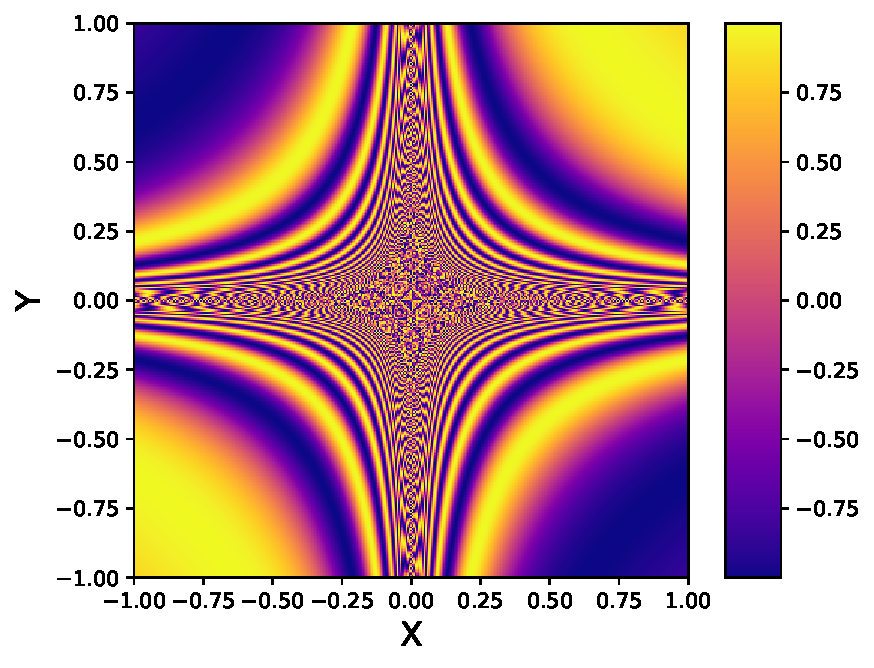
\includegraphics[width=0.5\linewidth]{figures/pretty_function.pdf}
    \oscaption{pretty_function}{%
        This is a plot of a pretty function. And at the end of this
        caption is a symbol with a link to the \emph{exact} script
        that generated it, hosted on \textsf{GitHub}.
        \label{fig:pretty_function}
    }
    \end{centering}
\end{figure}
%

Second, it defines the \textsf{\textbackslash proof} environment, which
adds a link to any equation pointing to a proof, derivation, or
verification of the equation in the form of a \textsf{Jupyter} notebook:
%
\begin{proof}{euler}
    \label{eq:euler}
    e^{i\pi} + 1 = 0.
\end{proof}
%
Check out \citet{Luger2018} for an example of a paper that uses these
features.

% Bibliography
\pagebreak
\bibliography{bib}

\end{document}
